\section{Evaluation}
\label{sec:eval}

The goal of this section is to address two research questions: 
First, we quantify the severity of \drop. 
Second, we evaluate the proposed detection mechanism's performance in terms of effectiveness and overhead. 
We start by describing the simulation model and set-up before detailing the simulation results and their interpretation for both research questions.


\subsection{Simulation Framework, Parameters and Metrics}
Our simulation framework relies on OSSim \cite{nguyen2013ossim}. 
OSSim is a packet level simulator for DONet \cite{zhang2005coolstreaming}, a pull-based online streaming overlay.
All our overlays use the network topology generator GT-ITM \cite{GT} with 1000 peers connected to 400 edge router. Furthermore, our simulation time is 500s and the presented results are averaged over 10 runs. 

We differentiate between malicious and benign peers when considering their online times. 
We assume that malicious peers join the overlay early and do not leave before the video dissemination ends in order to maximize their impact. 
In contrast,  benign peers joining is based on Pareto distribution, while their leaving times is estimated using Lognormal distributions, as motivated by real-world measurements \cite{distribution}.
Benign peers can rejoin the overlay in a uniform distribution around 10s. For both case studies, the streaming rate is $400kbps$, the chunk size $=2500B$ and the buffer size $=30s$.


% 
% \begin{table}[ht]
% \center
% \caption{Acronyms}
% \begin{tabular}{|c|c||c|c|}
% \hline
% 
% \bf{Var.} & \bf{Desc.}  & \bf{Var.} & \bf{Desc.} \\\hline\hline
% 
% mal. headnodes $\eta x$ & $\{5,8,10\}$ & chunk size & 2500B \\\hline
% sat. threshold $\satThres$ & $\{0.5,0.7,0.95\}$ & $\treply$ & 10s\\\hline
% mal. neighbors $MN$  & $\{0,15,24,70,100\}$ & stream Rate & 400kbps\\\hline
% min. responses $\minP$ &  $\{3,4\}$ & buffer size & 30s  \\\hline
% det. allowed $\minDR$ & 10 & list size $LS$ & $\{8,10\}$\\\hline
%   
% \end{tabular}
% \label{tab:parameters}
% \end{table}
% \vspace{-2.5mm}

The following metrics characterize the performance.
\subsubsection*{Satisfaction $\sat$} The satisfaction is the fraction of chunks peers receive in time, averaged over all peers. 
\subsubsection*{Avg. Loss $lo$} The average loss indicates the fraction of chunks that peers do not receive in time. 
\subsubsection*{Detection Overhead $DO$} The detection overhead describes the communication overhead created by the detection mechanism. More formally, it is the ratio of messages exchanged due to the detection mechanism and all signaling messages in the system.
\subsubsection*{Benign Ratio per Neighbor List $BRNL$} The benign ratio per neighbor list measures the fraction of benign peers in the source's neighbor list.

\subsection{Case 1: \drop Severity}

In this case study, we evaluate the impact of \drop on two different network scenarios:  (1) DONet, and (2) DONet+SWAP \cite{nguyen2016swap}. We consider SWAP to check how regular replacement of headnodes affects the attack. 
We use the same total number of peers but vary the attacker's budget.
As malicious peers aim to occupy the closest peers to the source, the remaining size of the overlay is not a factor on the impact of the \drop attack.

Given the source's neighbor list size $LS=10$, we choose the following combinations for the attackers budget $(eta x, MN)$: $(10,0), (5,15), (7,70), (8,24)$.
Here, $MN=70$ denotes that 7 malicious peers are connected to each of the 10 headnodes.
We start with analyzing the attack's impact on DONet and then we evaluate the resilience of SWAP to the attack.

Figure~\ref{subfig:avg-loss-donet} displays the average chunk loss ratio.
Unsurprisingly, the average loss is 100\% when $\eta x= LS =10$, which means that the source's $LS$ is utterly saturated with malicious headnodes, i.e., no chunks are transmitted to the rest of the overlay.
Thus,, the average peer satisfaction is always 0\%. 

If $\eta x < 10$, the average loss initially reaches up to ~82\% for $(\eta x, MN)=(7, 70)$, for $(\eta x, MN)=(5, 15)$, the loss ratio is ~54\% and ~73\% for $(\eta x, MN)=(8, 24)$, as shown in Figure~\ref{subfig:avg-loss-donet}.
If $\eta x$ or $MN$ increases, benign peers experience severe service degradation for a longer time period. 
Benign peers close to the source are overloaded with requests that they cannot respond to, leading to a high ratio of missed chunks. 
Nevertheless, the loss ratio decreases once a fraction of benign peers are able to serve the rest of the overlay.

Figure~\ref{subfig:satisfaction-donet} presents the average peer satisfaction level $\sat$.
As a consequence of experiencing high chunk loss rate, higher values of $\eta x, MN$ result in lower peer satisfaction over time, where benign peers at $(\eta x, MN)=(5, 15)$ restore their satisfaction level at ~340s, which is earlier than at $(\eta x, MN)=(7, 70)$ and $(\eta x, MN)=(8, 24)$.

Now we analyze the attack's impact while SWAP is operating.
During SWAP, peers nominate new headnodes and forward these nominations to the source. 
Malicious peers abuse the mechanism via nominating other malicious peers at each nomination round. 
Moreover, malicious peers connected to benign headnodes are eventually nominated to the source and thus can occupy the source's neighbor list $LS$. 

As shown in Figure~\ref{subfig:avg-loss-donet}, comparing the same values at $(\eta x, MN)=(5, 15)$ for both DONet and SWAP show that the impact of the attack is more significant if SWAP is active.
Before the source's $LS$ is saturated with malicious peers at $t=80s$, the average loss is in fact decreasing, However, as soon as malicious peers control the neighbor list, the average loss increases up to ~97\%. 
For the same reason, the satisfaction level of benign peers eventually decreases to ~6\%, which highlights the unsuitability of SWAP against our proposed attack.




\begin{figure}[tb]
%   \setlength{\belowcaptionskip}{-10pt}
  \centering
  \begin{subfigure}[c]{0.95\columnwidth}
    \centering
    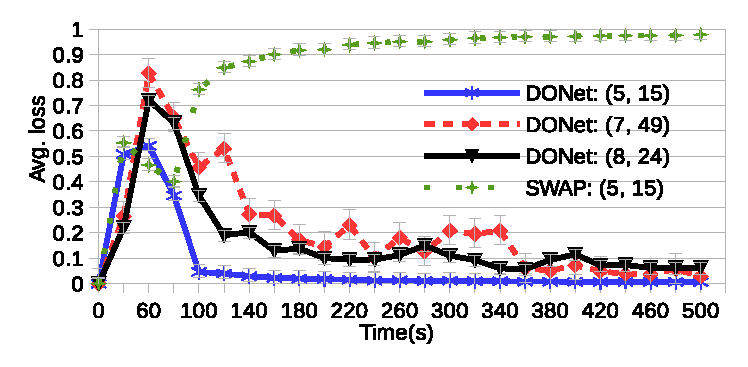
\includegraphics[width=8.4cm,height=3cm]{./Figures/avg-loss-donet.eps}
    \caption{Average loss}%
    \label{subfig:avg-loss-donet}
  \end{subfigure}
  \begin{subfigure}[c]{0.95\columnwidth}
    \centering
    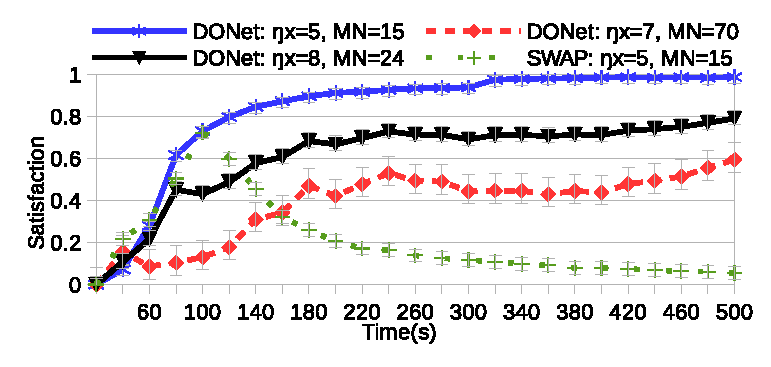
\includegraphics[width=8.4cm,height=3cm]{./Figures/satisfaction-donet.eps}
    \caption{Average peer satisfaction}%
    \label{subfig:satisfaction-donet}
  \end{subfigure}
  \caption{Attack's impact on DONet}%
  \label{fig:attack-results}
  \vspace{-7mm}
\end{figure}

% 
% 
% \begin{figure}[t!]
% \centering
% 
%   \mbox{\subfloat[Avg. loss]{\label{subfig:avg-loss-donet}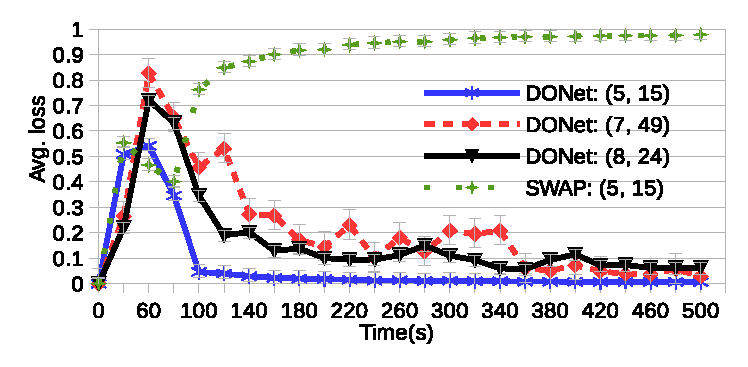
\includegraphics[width=8.4cm,height=3.5cm]{./Figures/avg-loss-donet.eps}}}
% %    \vspace{-3mm}
%   \mbox{\subfloat[Avg. peer satisfaction]{\label{subfig:satisfaction-donet}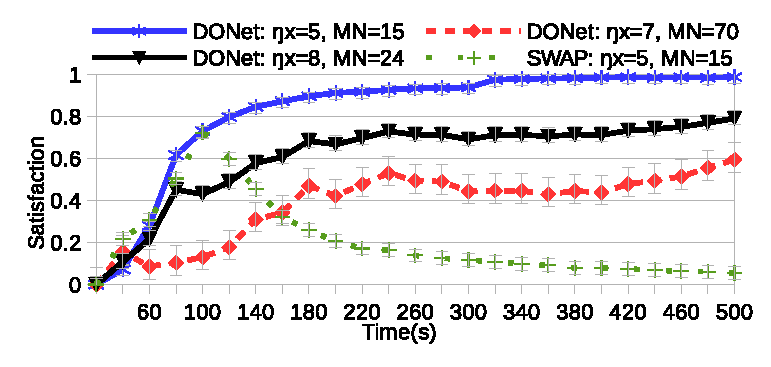
\includegraphics[width=8.4cm,height=3.5cm]{./Figures/satisfaction-donet.eps}}}
% %   \mbox{\subfloat[Avg. loss]{\label{subfig:avg-loss-donet}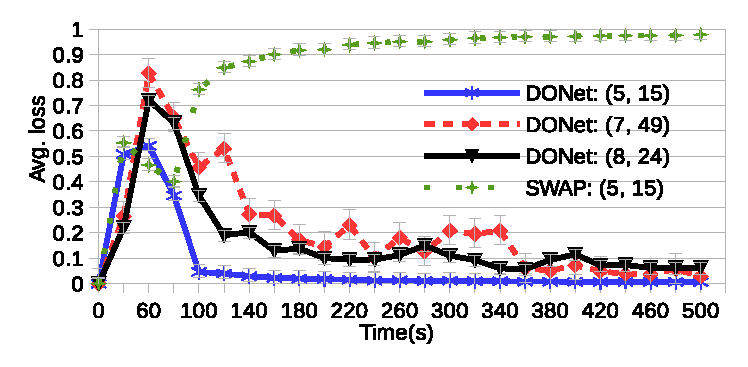
\includegraphics[width=3.7cm,height=2.5cm]{./Figures/avg-loss-donet.eps}} \subfloat[Avg. peer satisfaction]{\label{subfig:satisfaction-donet}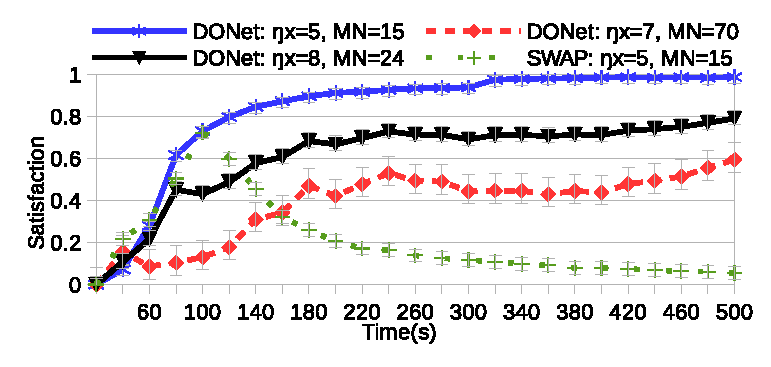
\includegraphics[width=3.7cm,height=2.5cm]{./Figures/satisfaction-donet.eps}}} 
% 
%   \caption{}
%   \vspace{-3.5mm}
%   \label{fig:attack-results}
%   \end{figure}
% 

\subsection{Case 2: Detection Mechanism Performance}


\begin{figure*}[tb]
%   \setlength{\belowcaptionskip}{-10pt}
  \centering
  \begin{subfigure}[t]{0.32\textwidth}
    \centering
    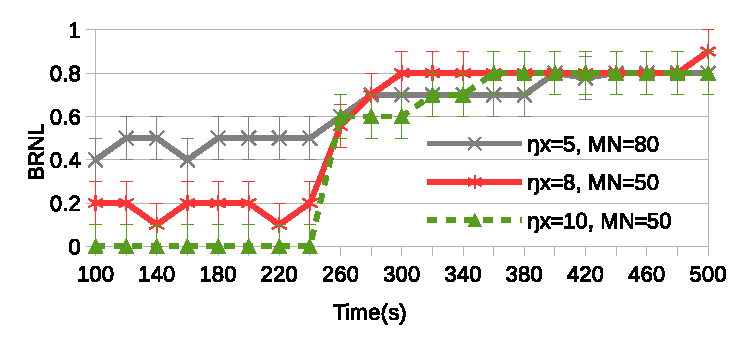
\includegraphics[width=6cm,height=3cm]{./Figures/det-BRNL1.eps}
    \caption{Average BRNL}%
    \label{subfig:BRNL}
  \end{subfigure}
  \begin{subfigure}[t]{0.32\textwidth}
    \centering
    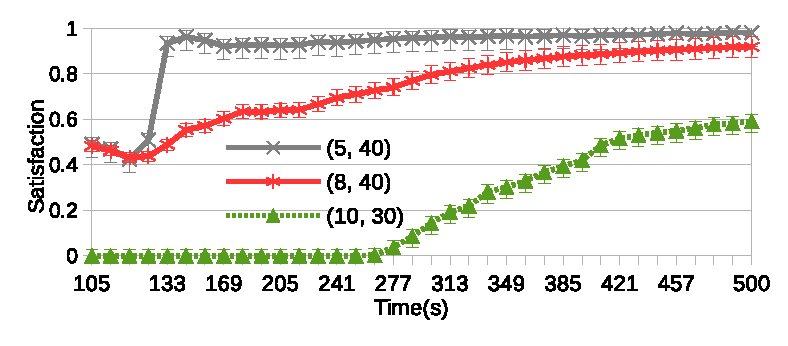
\includegraphics[width=6cm,height=3cm]{./Figures/det-sat.eps}
    \caption{Avg. peer satisfaction}%
    \label{subfig:det-sat}
  \end{subfigure}
  \begin{subfigure}[t]{0.32\textwidth}
    \centering
    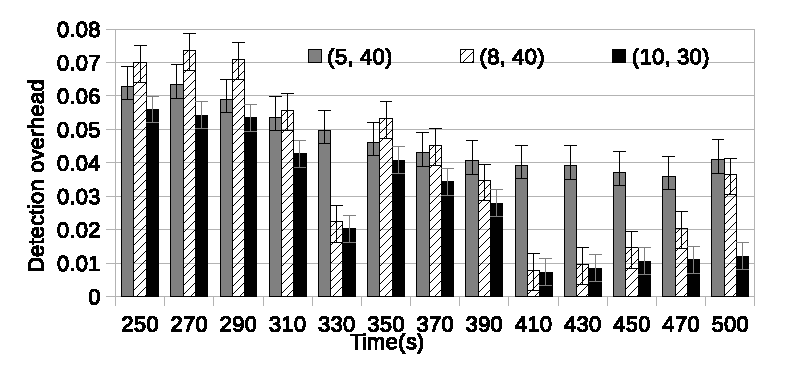
\includegraphics[width=6cm,height=3cm]{./Figures/overhead.eps}
    \caption{Detection overhead}%
    \label{subfig:overhead}
  \end{subfigure}
  \caption{Detection mechanism performance}%
  \label{fig:detection-results}
   \vspace{-4.5mm}
\end{figure*}


We now evaluate the performance of the detection mechanism.
Benign peers execute the detection mechanism as described in Section~\ref{sec:detection} whereas malicious peers aim to misuse the mechanism.
More precisely, malicious peers reply with a satisfaction level of 0 if the complaint might remove a benign peer and 1 if it might remove a malicious peer. 

In order to do so, we selected the following combinations for $(\eta x, MN)$: $(5, 80)$, $(8, 50)$ and $(10, 50)$ to assess the performance of the mechanism in severe attack conditions.
The satisfaction threshold $\satThres$ is set to 0.95 to measure if peers are able to fully restore their satisfaction level when the detection mechanism is operating.
The detection mechanism is effective starting $t=250s$ to allow for a reasonable amount of peers to join the overlay to adequately assess the efficiency of the mechanism.
In this scenario, every peer is allowed to initiate $\minDR=10$ detection requests for $t_{det}=500s$, and the minimum number of responses to generate a complaint is $\minP=3$. 
We discuss the effect of varying those parameters later on.

As depicted in Figure~\ref{subfig:BRNL}, once the detection mechanism is operating at $t=250s$, we observe an increase in the benign headnodes ratio in the source's neighbor list.
For instance, for $(\eta x, MN)=(5, 80)$, the source successfully attains ~80\% benign headnodes due to the detection mechanism.
For $(\eta x, MN)=(8, 50)$, the $BRNL$ ratio increases up to 90-100\%, which reflects the efficiency of the detection mechanism in replacing malicious headnodes to restore peers' satisfaction levels. 
Even if the source is initially only connected to malicious headnodes, i.e., $\eta x=10$, the detection mechanism is capable of restoring a $BRNL$ of close to 80\%. 

Figure~\ref{subfig:det-sat} illustrates the average restored peer satisfaction level due to the detection mechanism.
For the various attack placement strategies, the average satisfaction level increases up to ~95-100\%, even for $\eta x=10$.
As the detection mechanism starts at $t=250s$, the mechanism's impact on the peers' satisfaction level $\sat$ can be noticed in a short time period.
The reason is that the number of initial detection requests sent to the source results in replacing a high fraction of the source's headnodes and quickly increases the satisfaction levels. 
Moreover, malicious peers are unable to misuse the mechanism, as indicated by the absence of degradation in satisfaction levels. 

Figure~\ref{subfig:overhead} depicts the average detection overhead induced by our mechanism. 
The maximum overhead due to the detection mechanism is ~8\% for all scenarios.
As peers are eventually satisfied, the number of detection requests initiated decreases and the overhead decreases to ~4\% at $t=500s$, i.e., peers stop invoking the mechanism.
% This implies that the overhead is not constant throughout time, i.e., once all peers' satisfaction level exceeds $\satThres$, they do not invoke the detection mechanism and hence do not induce additional overhead. 
Moreover, the maximum number of detection requests that can be initiated is dependent on $\minDR$, which is set to 10 in this scenario.
Thus, smaller values of $\minDR$ result in lower overhead, which is a useful application parameter that can be set according to the application's criticality or the user's CPU resources.
In fact, varying $\minP$ between 3, 4 and 5 has little impact on the detection performance, indicating that nodes receive sufficient replies.

To that end, throughout the results, we highlight the efficiency of the detection mechanism against \drop attacks, even if the attacker possesses high malicious budget as headnodes.
% Moreover, we show that malicious peers are incapable of abusing the detection mechanism and place themselves as headnodes. Finally, the detection mechanism induces a very small overhead on the overlay.



% 
% \begin{figure*}[tb]
%   \centering
%   \begin{subfigure}[t]{0.32\textwidth}
%     \centering
%     \includegraphics[keepaspectratio]{fib-pass-114-rt}
%     \caption{$FIB$}%
%     \label{fig:anatime-fib}
%   \end{subfigure}%
%   \begin{subfigure}[t]{0.32\textwidth}
%     \centering
%     \includegraphics[keepaspectratio]{avl-max-pass-114-rt}
%     \caption{$AVL_{max}$}%
%     \label{fig:anatime-avl-max}
%   \end{subfigure}%
%   \begin{subfigure}[t]{0.32\textwidth}
%     \centering
%     \includegraphics[keepaspectratio]{avl-min-pass-114-rt}
%     \caption{$AVL_{min}$}%
%     \label{fig:anatime-avl-min}
%   \end{subfigure}
%   \caption{Time needed for the static analysis of the three synthetic test suites with varying number of test cases.
%            The colored upper part of the bars marks the time needed to apply the different subset search heuristics.}%
%   \label{fig:anatime-synwls}
% \end{figure*}




% \begin{figure}[t!]
% \centering
% \vspace{-3.5mm}
%   \mbox{\subfloat[Avg. BRNL]{\label{subfig:BRNL}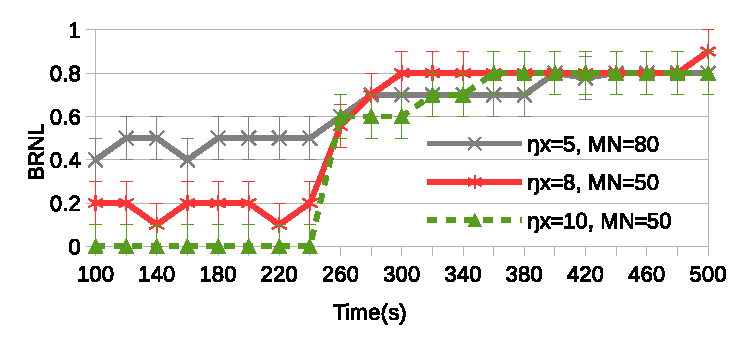
\includegraphics[width=8.4cm,height=3.5cm]{./Figures/det-BRNL1.eps}}}
% \vspace{-3.5mm}
%   \mbox{\subfloat[Avg. peer satisfaction]{\label{subfig:det-sat}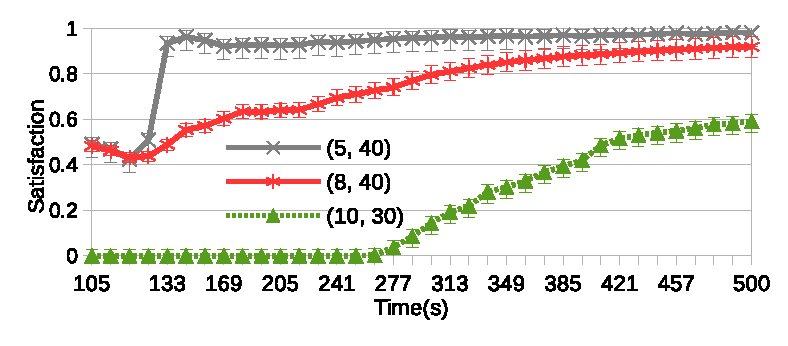
\includegraphics[width=8.4cm,height=3.5cm]{./Figures/det-sat.eps}}}
% 
%    \mbox{\subfloat[Detection overhead]{\label{subfig:overhead}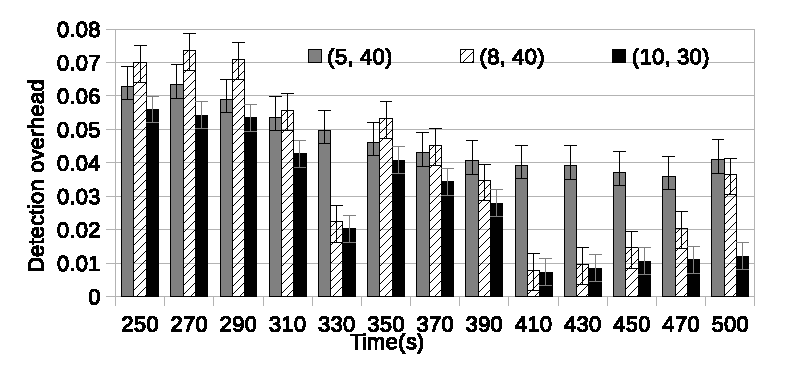
\includegraphics[width=8.4cm,height=3.5cm]{./Figures/overhead.eps}}}
% %   \vspace{-1.5mm}   
% %   \mbox{\subfloat[Avg. loss]{\label{subfig:avg-loss-donet}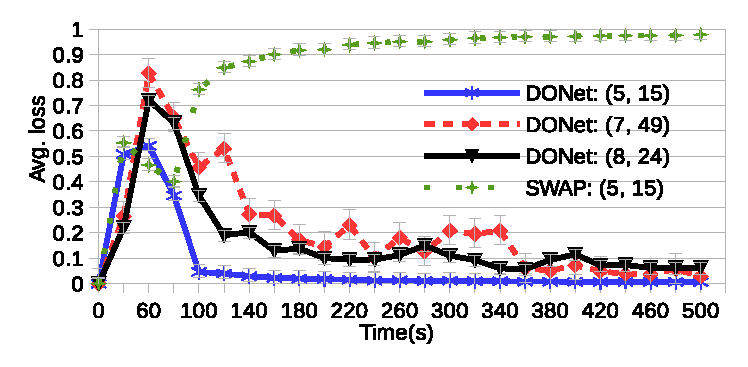
\includegraphics[width=3.7cm,height=2.5cm]{./Figures/avg-loss-donet.eps}} \subfloat[Avg. peer satisfaction]{\label{subfig:satisfaction-donet}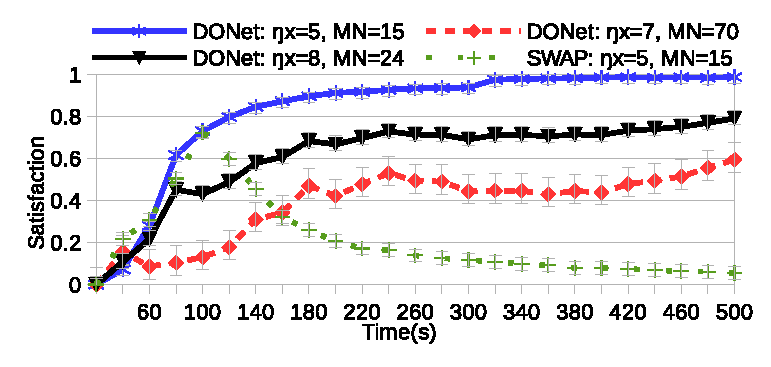
\includegraphics[width=3.7cm,height=2.5cm]{./Figures/satisfaction-donet.eps}}} 
% 
%   \caption{Detection mechanism performance}
%   \vspace{-3.5mm}   
%   \label{fig:detection-results}
%   \end{figure}


% \subsubsection{Summary of the results}
% 
% As a summary, for DONet, when the source's neighbor list is fully saturated with malicious peers, $IL$ is at ~100\%.
% Nevertheless, for smaller values of $Hx$, the attack's impact is still significantly high for a long period of time given the intolerability of such networks to such high delays.
% In fact, having only $Hx=\alpha$ without using $MN$ is sufficient for the attacker to completely isolate and thus, prevent the source from delivering any stream chunks.
% 
% For the SWAP case study, it is noticed that even with low values of $Hx$, after a certain swapping period, malicious peers manage to fully occupy the source's list and hence, $IL$ eventually reaches to ~100\%.
% This denotes that, the number of neighbors $MN$ is a major factor in the case of SWAP.
% Moreover, through an efficient distribution of the attacker's budget $x$, i.e., $Hx$ and $MN$, the attacker can decide whether to cause higher damage to the stream at the initialization time and then allow the network to eventually recover later on, or to allow the stream to reach to benign peers at earlier time phase till totally cutting the flow once $Hx=\alpha$ at some point.
